\begin{figure}
    \centering
    \begin{subfigure}[c]{0.48\linewidth}
        \centering
        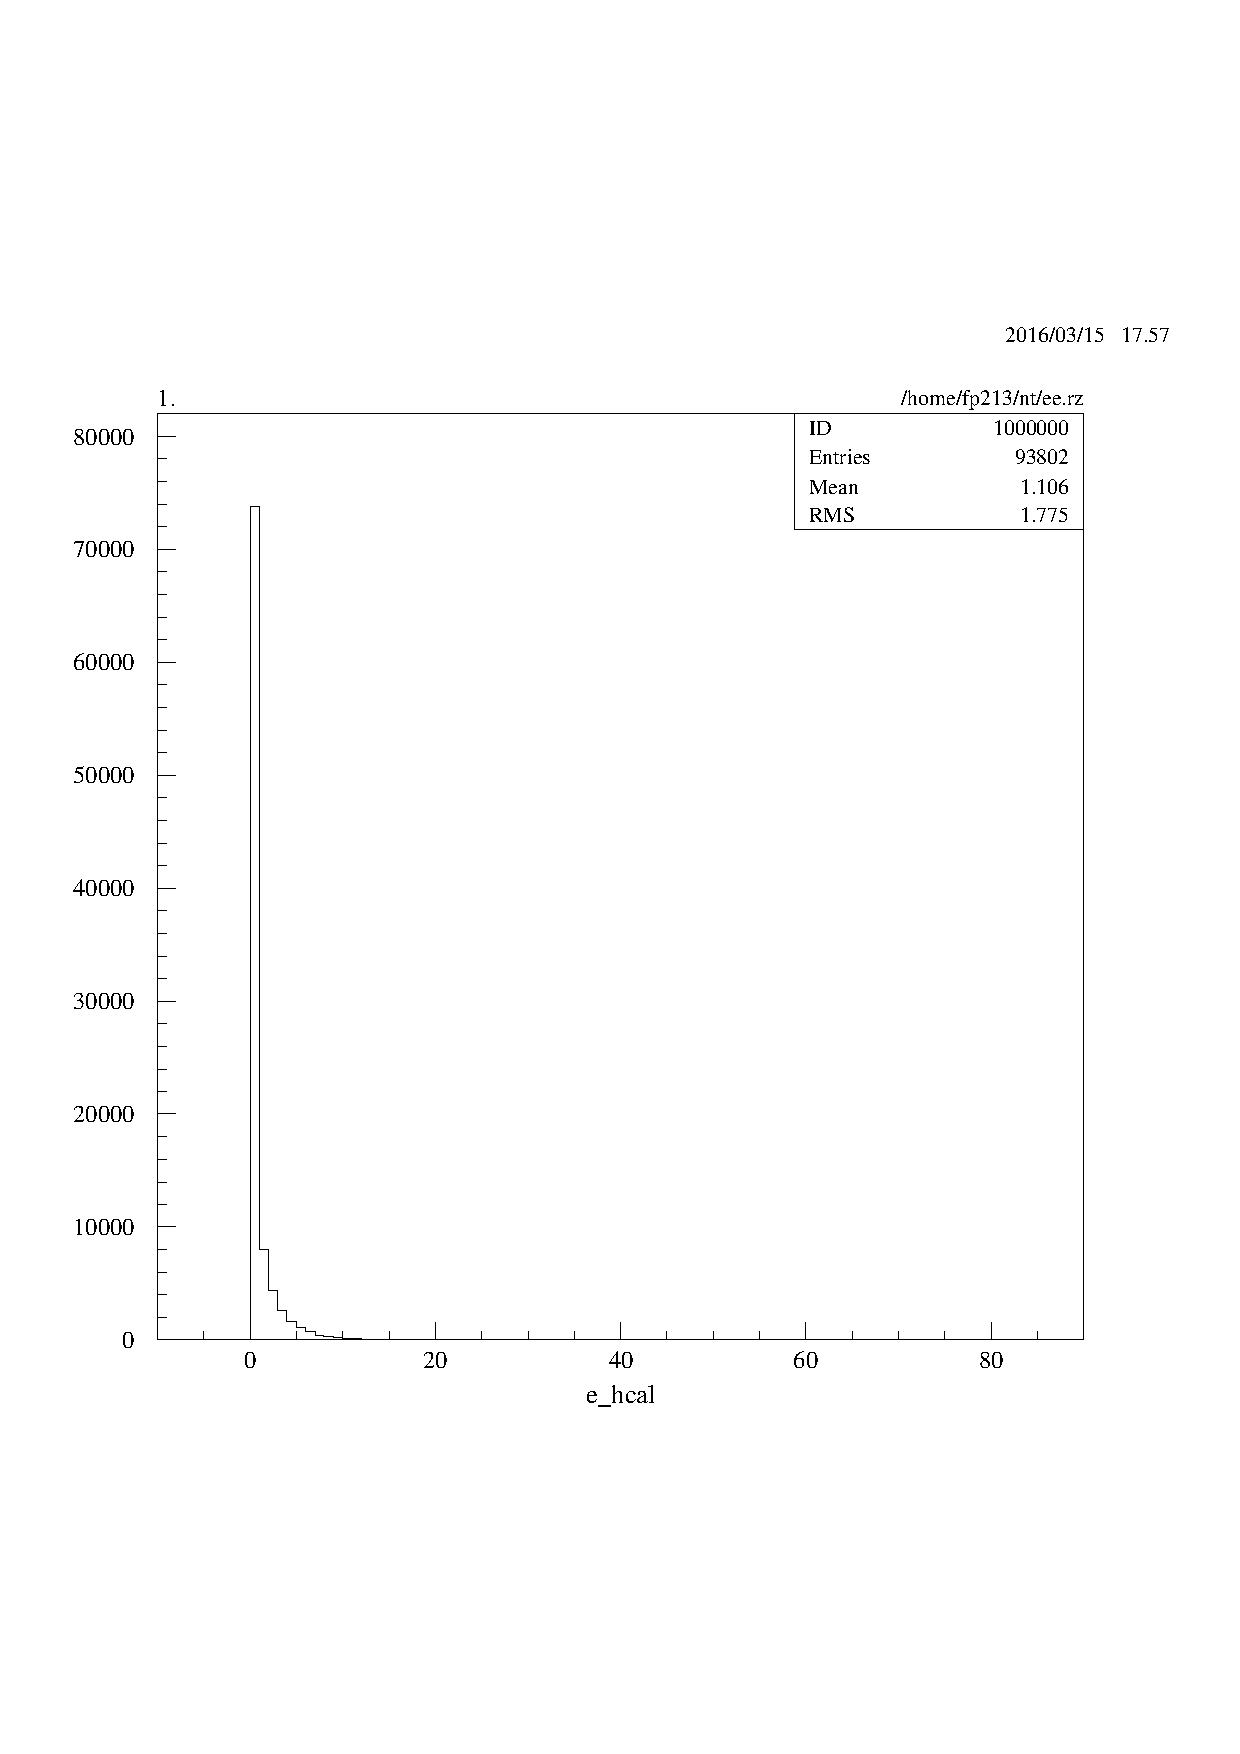
\includegraphics[width=\linewidth]{electrons-e_hcal}
        \caption{%
            Electrons
        }
        \label{fig:paw-e_hcal/electrons}
    \end{subfigure}
    \hfill
    \begin{subfigure}[c]{0.48\linewidth}
        \centering
        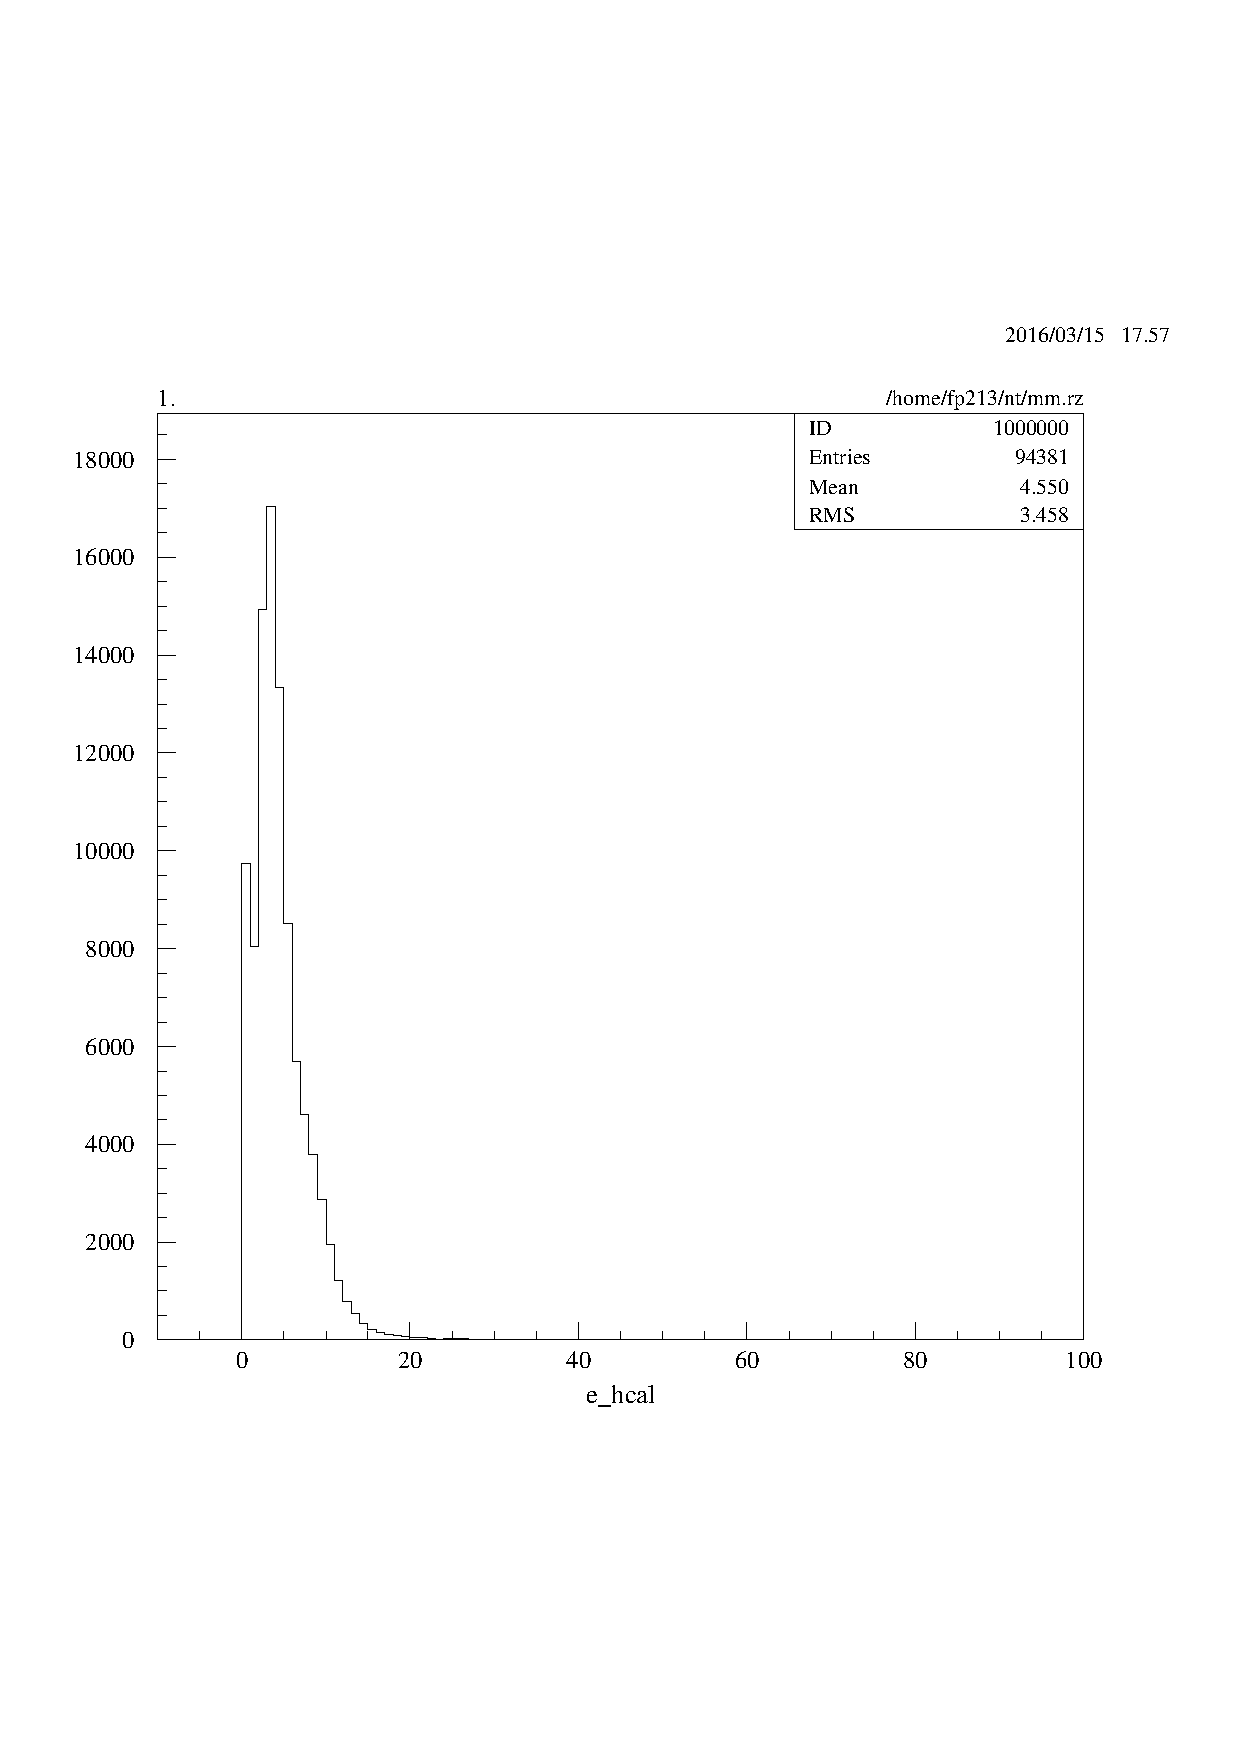
\includegraphics[width=\linewidth]{muons-e_hcal}
        \caption{%
            Muons
        }
        \label{fig:paw-e_hcal/muons}
    \end{subfigure}

    \vspace{2ex}

    \begin{subfigure}[c]{0.48\linewidth}
        \centering
        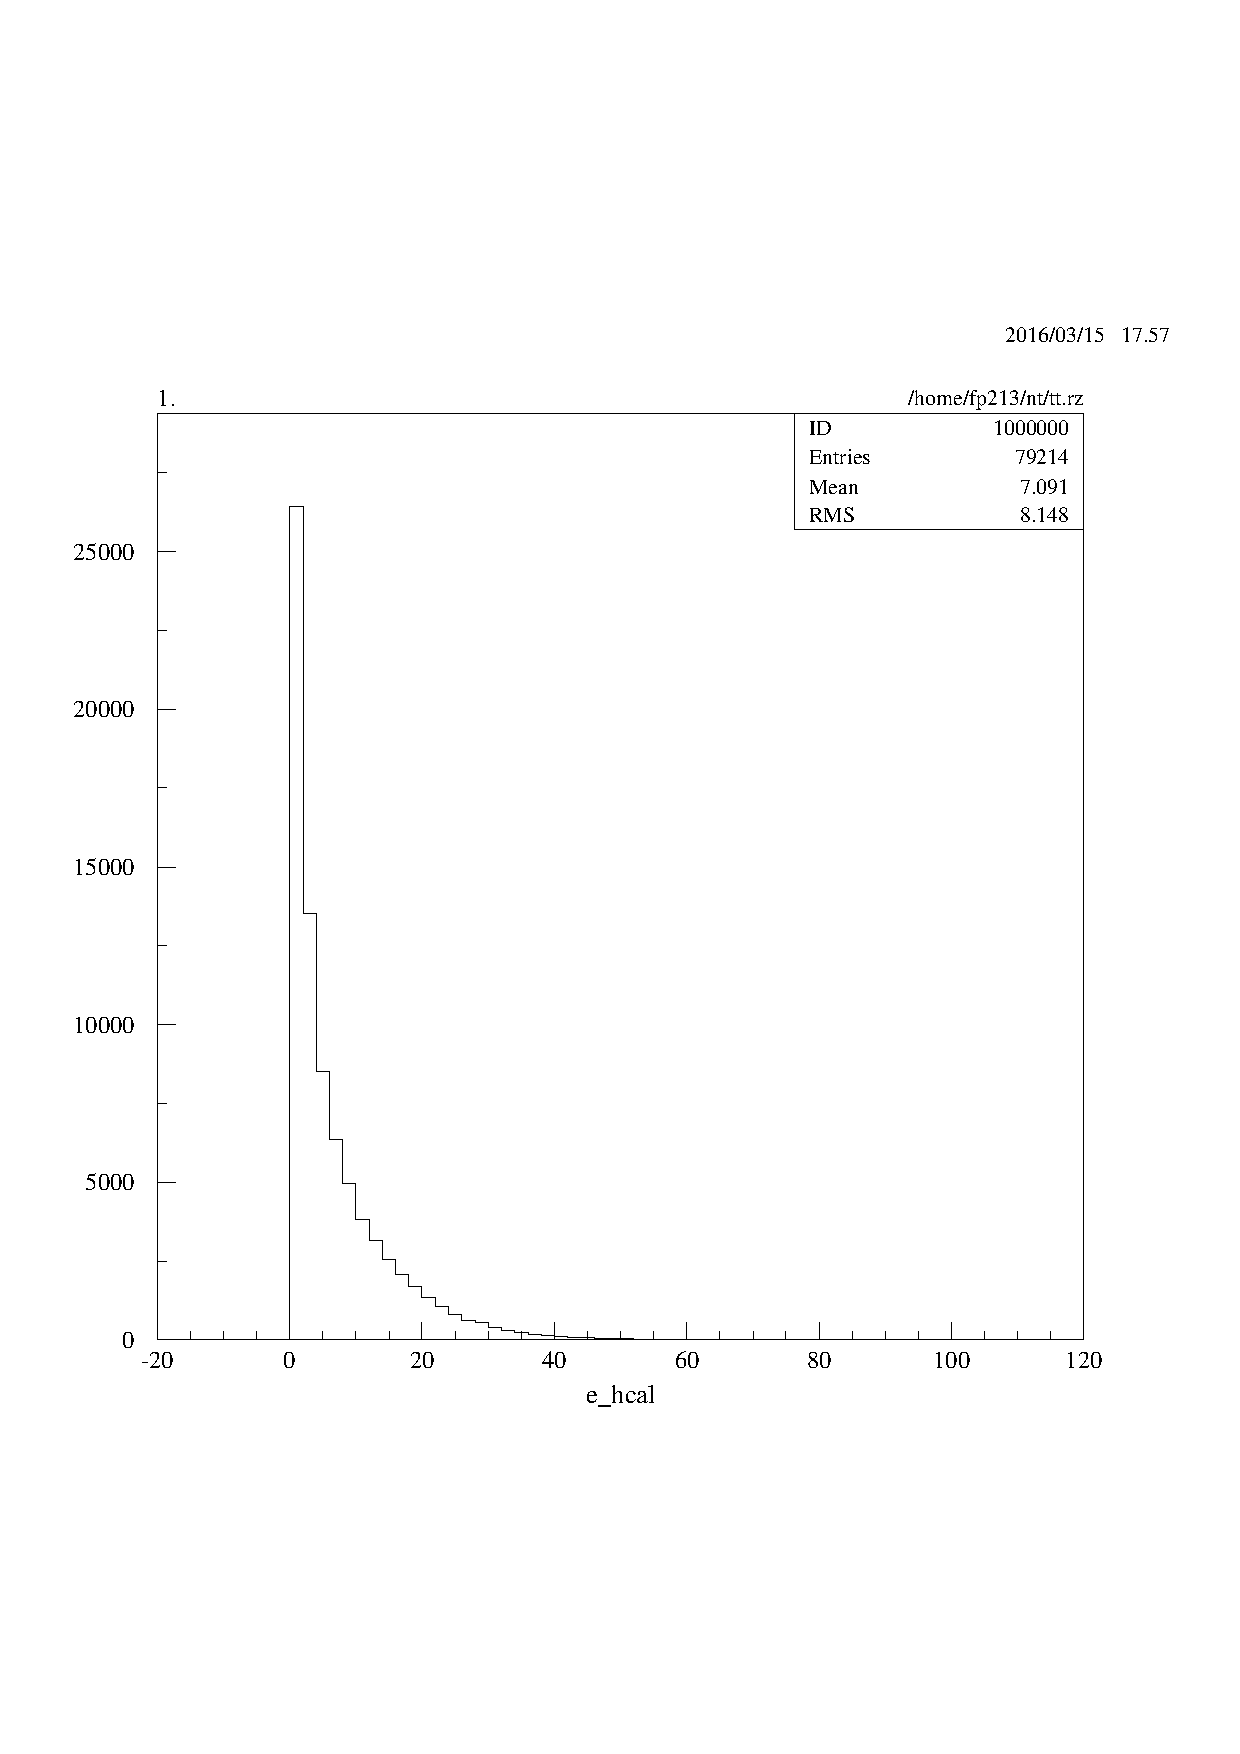
\includegraphics[width=\linewidth]{taus-e_hcal}
        \caption{%
            Taus
        }
        \label{fig:paw-e_hcal/taus}
    \end{subfigure}
    \hfill
    \begin{subfigure}[c]{0.48\linewidth}
        \centering
        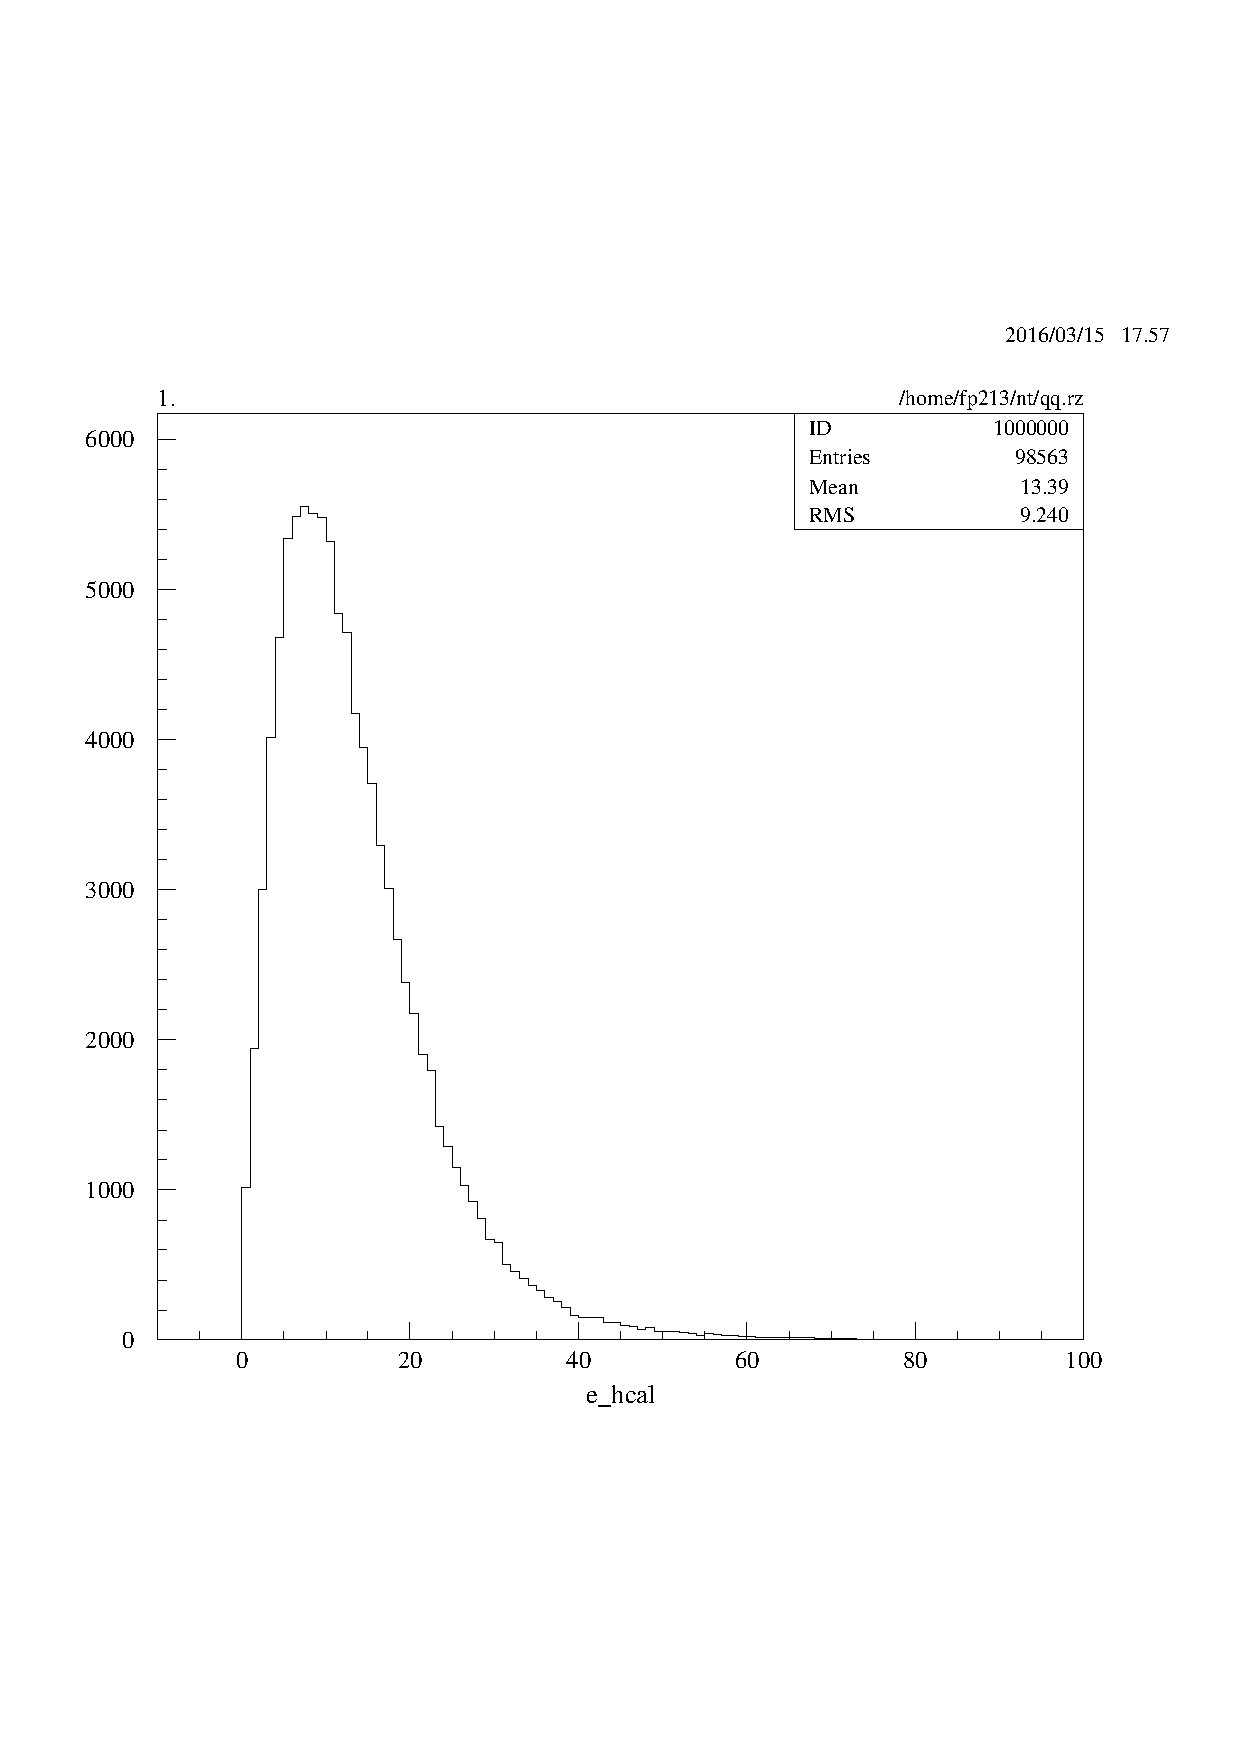
\includegraphics[width=\linewidth]{hadrons-e_hcal}
        \caption{%
            Hadrons
        }
        \label{fig:paw-e_hcal/hadrons}
    \end{subfigure}
    \caption{%
        Energy deposited into the \hcal\ for the four decay types.
        Histograms generated with \textsc{paw} from Monte Carlo datasets.
    }
    \label{fig:paw-e_hcal}
\end{figure}
